\documentclass[svgnames,11pt]{beamer}
\input{/home/tof/Documents/Cozy/latex-include/preambule_commun.tex}
\input{/home/tof/Documents/Cozy/latex-include/preambule_beamer.tex}
%\usepackage{pgfpages} \setbeameroption{show notes on second screen=left}
\author[]{Christophe Viroulaud}
\title{Publier une page web}
\date{\framebox{\textbf{Web 03}}}
%\logo{}
\institute{Seconde - SNT}

\begin{document}
\begin{frame}
    \titlepage
\end{frame}
\begin{frame}
    \frametitle{}

    Les pages web créées ne sont accessibles que depuis la machine utilisée pour la création.
    \begin{framed}
        \centering Comment rendre une page web publique?
    \end{framed}

\end{frame}
\section{Publier}
\begin{frame}
    \frametitle{Publier}

    \begin{center}
        \centering
        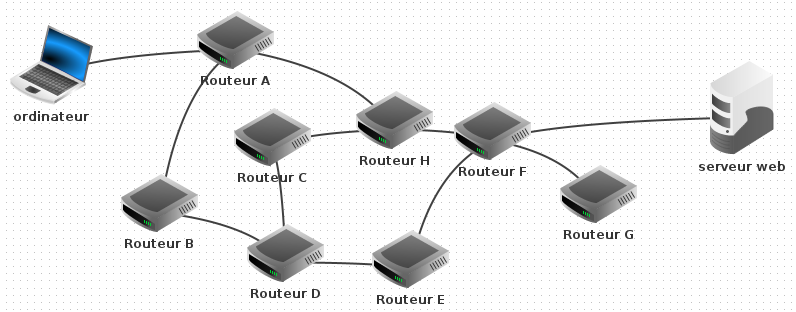
\includegraphics[width=9cm]{ressources/serveur-web.png}
        \captionof{figure}{\centering Le réseau Internet relie tous les ordinateurs entre eux}
        \label{IMG}
    \end{center}

\end{frame}
\begin{frame}
    \frametitle{}

    \begin{center}
        \centering
        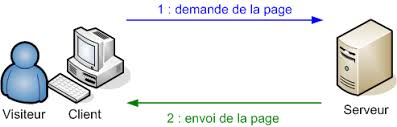
\includegraphics[width=8cm]{ressources/http.jpeg}
        \captionof{figure}{\centering Certaines machines ont un rôle particulier: \textbf{les serveurs}.}
        \label{IMG}
    \end{center}

\end{frame}
\begin{frame}
    \frametitle{}
    \begin{center}
        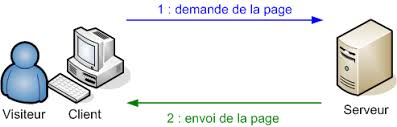
\includegraphics[width=6cm]{ressources/http.jpeg}
    \end{center}
    \begin{aretenir}[]
        Un serveur est un ordinateur toujours allumé et qui stocke des pages web. Un navigateur interroge un serveur pour récupérer une page web.
    \end{aretenir}

\end{frame}
\begin{frame}
    \frametitle{}

    Chaque page web possède une adresse unique: \textbf{URL: Uniform Resource Locator}
    \begin{center}
        {\Large https://cviroulaud.github.io/sites/viroulaud}
    \end{center}

\end{frame}
\begin{frame}
    \frametitle{}

    \begin{itemize}
        \item<1-> \textbf{http:} protocole du web
        \item<2-> http\textbf{s}: version sécurisée du protocole
        \item<3-> \textbf{cviroulaud.github.io:} nom de domaine
        \item<4-> \textbf{sites/viroulaud:} chemin vers la ressource
    \end{itemize}

\end{frame}
\section{Sécuriser}
\subsection{Définition}
\begin{frame}
    \frametitle{Sécuriser - Définition}

    \begin{center}
        \centering
        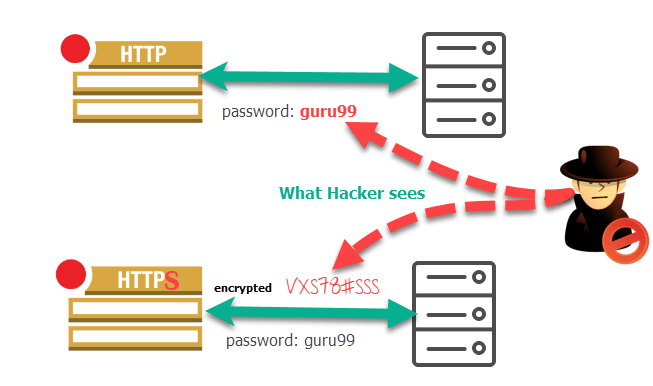
\includegraphics[width=8cm]{ressources/secure.png}
        \captionof{figure}{\centering Si la page web est sécurisée, \underline{toutes} les données transmises sont chiffrées.}
        \label{IMG}
    \end{center}
\end{frame}
\begin{frame}
    \frametitle{}

    \begin{activite}
        \begin{enumerate}
            \item Le site \url{https://cviroulaud.github.io/} est-il sécurisé? Comment le sait-on?
            \item Quel organisme a délivré le certificat de sécurité pour ce site?
        \end{enumerate}
    \end{activite}

\end{frame}
\begin{frame}
    \frametitle{Correction}

    \begin{center}
        \centering
        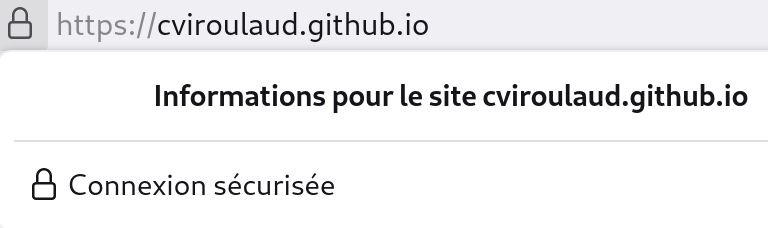
\includegraphics[width=8cm]{ressources/certificat.png}
    \end{center}
    \begin{aretenir}[]
        \begin{itemize}
            \item Le \textbf{s} du \emph{https} indique que la page est sécurisée.
            \item Les certificats de sécurité sont distribués par des organisme spécialisés.
        \end{itemize}
    \end{aretenir}
\end{frame}
\begin{frame}
    \frametitle{}

    \begin{activite}
        \begin{enumerate}
            \item Ouvrir une fenêtre de navigation privée dans le navigateur.
            \item Comment reconnaît-on que la page est en mode privé?
            \item Quel est le rôle du mode privé?
            \item Le mode privé prévient-il lors du téléchargement accidentel d'un virus? Qui joue normalement ce rôle dans un ordinateur?
        \end{enumerate}
    \end{activite}

\end{frame}
\begin{frame}
    \frametitle{Correction}

    \begin{aretenir}[]
        \begin{itemize}
            \item Le mode privé ne conserve pas les données de navigation (historique, cookies\dots)
            \item Par contre il ne garantit pas la sécurité des transmissions.
        \end{itemize}
    \end{aretenir}

\end{frame}
\subsection{Page non sécurisée}
\begin{frame}
    \frametitle{Page non sécurisée}

    \begin{activite}
        \begin{enumerate}
            \item Ouvrir le navigateur Firefox.
            \item Se rendre sur le site \url{http://jay.info.free.fr}
            \item Entrer un identifiant et un mot de passe fictifs. \textbf{Ne pas valider tout de suite.}
            \item  Cliquer sur \textbf{Ctrl+Shift+E}, le panneau \textbf{réseau} s'ouvre.
            \item Dans la page web, valider le formulaire.
            \item Ouvrir la ligne \textbf{POST}:
                      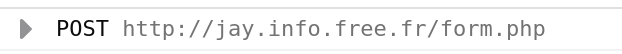
\includegraphics[width=9cm]{ressources/post-ff.png}
            \item Dans \textbf{Requêtes}, retrouver alors les informations transmises.
        \end{enumerate}
    \end{activite}

\end{frame}
\begin{frame}
    \frametitle{}

    \begin{aretenir}[]
        Sur un site non sécurisé, les informations sont transmises \textbf{en clair} entre les pages. Il est alors possible d'intercepter les données facilement.
    \end{aretenir}

\end{frame}
\subsection{Force d'un mot de passe}
\begin{frame}
    \frametitle{Force d'un mot de passe}

    \begin{activite}
        \begin{enumerate}
        \item Lire l'article sur la page \url{https://tinyurl.com/mot-passe}
        \item Quel est le mot de passe le plus populaire en 2020?
        \item Que peut-on dire du niveau de sécurité des mots passes les plus utilisés?
        \item Se rendre sur le site \url{https://tinyurl.com/force-passe}
        \item Calculer la force des mots de passe suivants:
        \begin{itemize}
        \item 12345678
        \item ABUEODNORR
        \item AQIU12N9
        \item AsSoI904nU12
        \item A\%2sIP9\#Bb
        \end{itemize}
        \end{enumerate}
        \end{activite}

\end{frame}
\begin{frame}
    \frametitle{Correction}
\begin{aretenir}[]
Un mot de passe \textbf{fort} est impératif pour protéger correctement les données. Il doit:
\begin{itemize}
    \item être long,
    \item contenir différents types de caractères,
    \item ne pas contenir d'information personnelle.
\end{itemize}
\end{aretenir}
    
    \begin{itemize}
        \item 12345678 $\;\rightarrow\;$27
        \item ABUEODNORR $\;\rightarrow\;$47
        \item AQIU12N9$\;\rightarrow\;$32
        \item AsSoI904nU12 $\;\rightarrow\;$68
        \item A\%2sIP9\#Bb$\;\rightarrow\;$61
        \end{itemize}
\end{frame}
\begin{frame}
    \frametitle{}

    \begin{activite}
        Dans Pix, réaliser la compétence \textbf{Sécuriser l'environnement numérique}.
        \end{activite}

\end{frame}
\end{document}